%%%%%%%%%%%%%%%%
\chapter{Out-of-equilibrium interfaces}
%%%%%%%%%%%%%%%%
We consider the effect of uniform driving on the interface between two phases which are described by model C dynamics. The non-driven system has a classical Gaussian interface described by capillary wave theory. The model under driving retains Gaussian statistics but the interface statistics are modified by driving, notably the height fluctuations are suppressed and  the correlation length of the fluctuations is increased.

%%%%%%%%%%%%%%%%
    \section{Introduction}
%%%%%%%%%%%%%%%%

The model we introduce can also be used as a model for the effect of activity on interface dynamics.
One of the most natural ways of creating a non-equilibrium steady state is by applying external  driving forces. Driving arises naturally in sedimenting systems due to gravity, in systems with free charges under the action of an electric field and also  due to the radiation pressure exerted by a laser. Experiments where a phase separated colloidal system is sheared parallel to the interface show that  driving due to shear tends to suppress surface fluctuations \cite{derks_suppression_2006}, and similar results are found where Ising models are numerically sheared  \cite{smith_interfaces_2008-1,smith_driven_2010}. These results are somewhat surprising, for instance they are contrary to the  observation that wind generates waves on the ocean. One may think that the precise nature of the driving plays a role, for instance uniformly driving a system may be intrinsically different to applying a shear field which is manifestly nonuniform. In this paper we investigate analytically the effect of uniform driving on a simple interface model. We find that the effect of this type of  driving is also to reduce surface fluctuations.

Constructing a continuum model which is analytically tractable and is also affected by uniform driving is straightforward but contains some subtleties. In a continuum system it is clear that uniform driving can only move a system away from equilibrium when the driving acts differently on different particle types. For instance, consider  a system of identical interacting Brownian particles driven by a uniform  force. The force will induce the same average velocity on all the particles, consequently, in the frame moving with this average velocity, we will recover the unmodified equilibrium state. However, when multiple particle types are present, the mean velocity induced on different species are different and no Galilean transformation is possible. Perhaps the first such study of this phenomenon was due to Onsager \cite{lars_onsager_collected_1996}, who studied the conductivity of electrolytes and in doing so showed how the correlation functions in the steady state were modified by the electric field. 
Recently there have been many studies of driven multi-particle Brownian systems \cite{dzubiella_lane_2002,chakrabarti_dynamical_2003,chakrabarti_reentrance_2004,sutterlin_dynamics_2009,glanz_nature_2012, klymko_microscopic_2016}, including the electrolyte problem,  and rich new physics has been found, even in the case of purely Gaussian theories \cite{demery_conductivity_2016,poncet_universal_2017} based on stochastic density functional theory \cite{dean_renormalization_1996}. 

The dynamics of discrete particle systems is however affected by uniform driving of identical particles. The study of driven lattice gases has revealed a wide range of intriguing physical phenomena and indeed shown how driving can even lead to phase separation \cite{katz_nonequilibrium_1984,zia_interfacial_1991,leung_anomalous_1993,schmittmann_driven_1998}. The discrete nature of the dynamics of these systems, both in space and time, means that no Galilean transformation to an equilibrium state exists. Analytical studies of these systems require a phase ordering kinetics description in terms of a continuum order parameter. In order to break Galilean invariance the local mobility of the particles can be taken to be dependent on the local order parameter, this is then sufficient to induce non-trivial steady states under driving \cite{katz_nonequilibrium_1984,leung_anomalous_1993,smith_interfaces_2008,smith_lateral_2010}. Interfaces between the separated phases in uniformly driven systems have non capillary behaviors which are, even today, not fully understood \cite{leung_anomalous_1993}.
Taking random driving in a given direction also leads to non-equilibrium steady states, if the noise is Gaussian and white, the fluctuation dissipation theorem is violated and novel interface fluctuations are induced which, again, are  not of  the capillary type \cite{zia_interfacial_1991}. 

Driving can also be deterministic but space dependent, for instance if one considers applied shear flows, the spatial dependence of the flow means no Galilean transformation to an equilibrium steady state is possible and this therefore leads to non-equilibrium steady states. The effect of shear on interfaces in these type of systems yields interface equations of the stochastic Burgers type and the statistics are no thus longer Gaussian due to the presence of nonlinearities \cite{bray_interface_2001,bray_interface_2001-1,smith_interfaces_2008,smith_lateral_2010,thiebaud_nonequilibrium_2010,thiebaud_nonlinear_2014}


In this paper we analyse what is known, in the classification of Hohenberg and Halperin \cite{hohenberg_theory_1977}, as model C type dynamics for two fields, one with conserved model B type dynamics, which is in addition convected at a uniform velocity to mimic driving. We refer to this first field as the colloid field.
This colloid field is coupled to an additional field which undergoes model A non-conserved dynamics and which is not subjected to the driving. The model A field can be thought of a passive solvent and its coupling to the model B field is chosen in such a way that it has no influence on the non-driven equilibrium steady state. We then derive the effective dynamics between two separated low temperature phases by using a
method introduced in \cite{bray_interface_2001,bray_interface_2001-1} for the study of interfaces under shear flow. This method yields a Gaussian theory for the interface statistics and driving introduces interesting new physics, notably we find that the effective surface tension of the system is increased but also the correlation length of interface fluctuations (due to an effective gravitational term) are increased. These observations are in qualitative agreement with experimental results on sheared low tension interfaces in phase separated colloidal systems \cite{derks_suppression_2006}. In this experimental system the interface fluctuations were also found to be well described by Gaussian statistics and this is our principal motivation for studying theories which remain Gaussian but are  modified by driving. While the long wavelength theory we find is of a capillary type, we also find new, higher derivative terms, which  are generated in the spectrum of the height fluctuations. 

As an aside, we also show how the model introduced here can be used to analyse the effect of activity on the dynamics of the surface between two phases of active colloids. The activity is implemented by taking a different temperature for the colloid and solvent fields, this difference in temperatures leads to significantly modified surface statistics which again develop dependencies on static and dynamical variables of the model which otherwise remain hidden for the equilibrium version of the problem.

%%%%%%%%%%%%%%%%
    \section{Driven model C interfaces}
%%%%%%%%%%%%%%%%

%%%%%%%%%%%%%%%%
    \subsection{The underling two field  model}
%%%%%%%%%%%%%%%%

We consider a coarse grained model for two scalar fields $\psi$ and $\phi$ with Hamiltonian
\begin{equation}
    H[\psi,\phi] = H_1[\psi] +H_2[\psi,\phi]
\end{equation}
The Hamiltonian $H_1$ is of the classic Landau-Ginzburg form
\begin{equation}
    H_1[\psi]=\int d\bx\left[\frac{\kappa}{2}[\nabla\psi(\bx)]^2 + V(\psi(\bx))
- gz \psi(\bx)\right]
\end{equation}
The last term represents the energy due to a gravitational field and will introduce a finite correlation length in the fluctuations between the two phases. We assume that the above Hamiltonian has two stable phases with average concentrations of the field $\phi(\bx)$ given by the constant values $\psi_1$ and $\psi_2$, the difference between the order parameter in  the two different phases is denoted by 
by $\Delta\psi= \psi_2 -\psi_1 \greater 0$. This means that we find the phase $1$ as $z\to\infty$ and the phase $2$ as $z\to-\infty$. The term $H_2$ is taken to be a simple quadratic coupling between the fields
\begin{equation}
    H_2 =\int d\bx \frac{\lambda}{2}(1-\psi(\bx)-\phi(\bx))^2
\end{equation}
which is an approximative conservation law of total volume fraction of the phases. The field $\phi$ can be though of as the local volume fraction of the solvent in a colloidal system. However the presence of this solvent field does not change the effective equilibrium statistical mechanics of the colloid field $\psi$ as the partition function can be written as 
\begin{equation}
    Z = \int d[\phi]d[\psi]\exp(-\beta H_1[\psi]- \beta H_2[\psi,\phi]) = CZ_{eff}
\end{equation}
where $Z_{eff}$ is the effective partition function for the field $\psi$, after we have integrated out the degrees of freedom corresponding to the field $\phi$,
and $C$ is a constant term resulting from this integration. The effective partition function is thus simply given by
\begin{equation}
    Z_{eff} = \int d[\psi]\exp(-\beta H_1[\psi])
\end{equation}
and, as stated above, we see that the field $\phi$ thus has no effect on the equilibrium statistical mechanics of the field $\psi$.

\begin{figure}
    \centering
    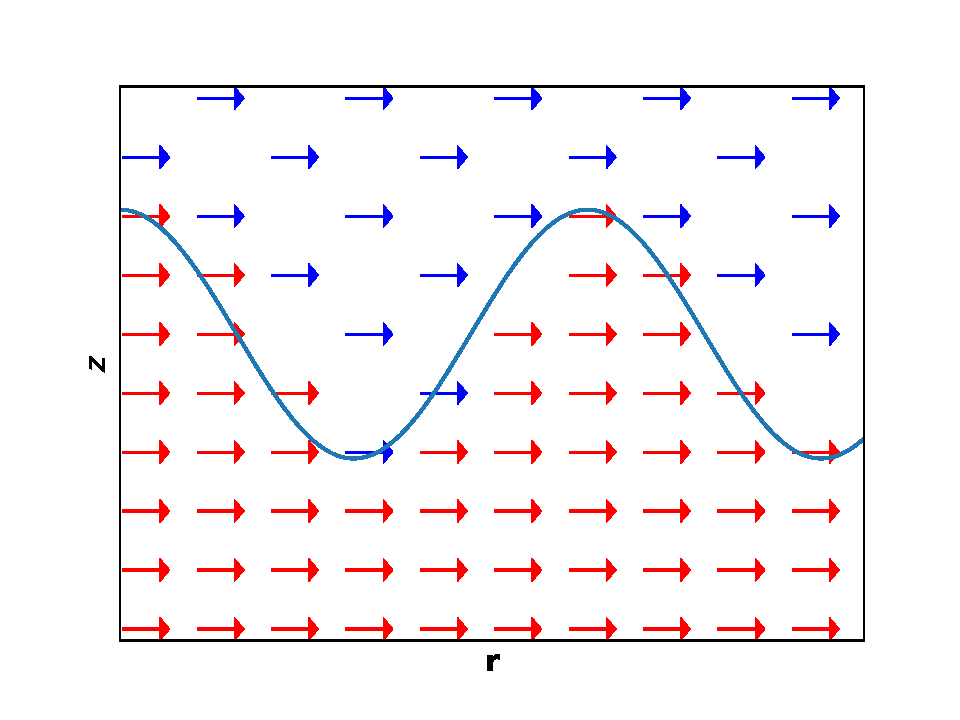
\includegraphics[width=0.7\linewidth]{drivenC/driven.pdf}
    \caption{Schematics of the advection term ${\bf v}\cdot { \nabla}\psi(\bx,t)$ for a field under the interface approximation \eqref{dynamical-interface}. The red and blue phase respectively correspond to $\phi_2$ and $\psi_1$, with $\phi_2 \greater \psi_1$, and the solid line the interface between phases.}
    \label{fig-driven}    
\end{figure}

We now consider the dynamics of the fields. We take local diffusive model B dynamics for the field $\psi$ and non-conserved model A dynamics for the field $\phi$
\begin{eqnarray}
\frac{\partial \psi(\bx,t)}{\partial t} +{\bf v}\cdot { \nabla}\psi(\bx,t)&=& D\nabla^2\frac{\delta H}{\delta \psi(\bx)}+ \sqrt{2D T}\nabla \cdot {\bm \eta}_1(\bx,t) \\
\frac{\partial \phi(\bx,t)}{\partial t} &=& -\alpha\frac{\delta H}{\delta \phi(\bx)}+ \sqrt{2\alpha T}{ \eta}_2(\bx,t).
\end{eqnarray}
The first equation corresponds to standard model B dynamics but with an advection term by a constant velocity field $\bf v$. 
{\color{red} In Fig \ref{fig-driven}, we show the effect of that advection term in the presence of an interface. Since phase 1 is more diluted than phase 2, there are less particles which are driven at constant velocity $\bv$.}
The second equation has no advection term and is simple model A dynamics. In principle we can also treat the case where the dynamics of the field $\phi$ is also diffusive and thus of model $B$ type, the analysis given here can be extended to this case but the analysis of the resulting equations is considerably more complicated. The use of model A dynamics for the solvent is justified by assuming that its dynamics is faster than that of the colloids and that the volume fraction can vary due to local conformational changes rather than  diffusive transport.

The noise terms above 
are uncorrelated and Gaussian with zero mean, their correlation functions are given by
\begin{eqnarray}
< \eta_{1i}(\bx,t) \eta_{1j}(\bx',t)>&=& \delta_{ij}\delta(t-t') \delta(\bx-\bx') \\
< \eta_{2}(\bx,t) \eta_{2}(\bx',t)>&=& \delta(t-t') \delta(\bx-\bx') ,
\end{eqnarray}
and $T$ is the temperature in units where $k_B=1$.
These dynamical equations  are thus explicitly given by
\begin{equation}
    \frac{\partial \psi(\bx,t)}{\partial t} +{\bf v}\cdot { \nabla}\psi(\bx,t)= D\nabla^2[\frac{\delta H_1}{\delta \psi(\bx)}+\lambda(\phi(\bx,t) + \psi(\bx,t))]+ \sqrt{2D T}\nabla \cdot {\boldsymbol \eta}_1(\bx,t)
\end{equation}
and
\begin{equation}
    \frac{\partial \phi(\bx,t)}{\partial t} = -\alpha\lambda[\phi(\bx,t) + \psi(\bx,t)]+ \sqrt{2\alpha T}{ \eta}_2(\bx,t).
\end{equation}
Taking the temporal Fourier transform, defined with the convention
\begin{equation}
    \tilde F(\bx, \omega) = \int_{-\infty}^\infty dt \exp(-i\omega t)F(\bx, t),
\end{equation}
we can eliminate the field $\tilde \phi$ which is given by
\begin{equation}
    \tilde \phi(\bx,\omega) = \frac{-\alpha\lambda \tilde \psi(\bx,\omega)+\sqrt{2\alpha T}\tilde \eta_2(\bx,\omega)}{i\omega +\alpha \lambda},
\end{equation}
this then gives the closed equation for $\tilde \psi$:
\begin{equation}
    \left[1-\frac{\lambda D \nabla^2}{i\omega+\alpha\lambda}\right]i\omega \tilde\psi(\bx, \omega) +{\bf v}\cdot\nabla\tilde\psi(\bx, \omega)
= D\nabla^2 \tilde \mu(\bx,\omega) +  \tilde \zeta(\bx,\omega),
\end{equation}
where 
\begin{equation}
    \mu(\bx,t)=\frac{\delta H_1}{\delta \psi(\bx,t)}
\end{equation}
is the effective chemical potential associated with the field $\psi$ and the noise term is given by
\begin{equation}
    \tilde \zeta(\bx,\omega) = \frac{\sqrt{2\alpha T}D\lambda}{i\omega + \alpha\lambda}\nabla^2\tilde \eta_2(\bx,\omega) +
\sqrt{2DT}\nabla\cdot\tilde {\bm \eta}_1(\bx,\omega).
\end{equation}
Inverting the temporal Fourier transform then gives the effective evolution equation
\begin{equation}
    \frac{\partial \psi(\bx,t)}{\partial t} -\lambda D\nabla^2\int_{-\infty}^t dt'
\exp(-\alpha\lambda(t-t')) \frac{\partial \psi(\bx,t')}{\partial t}+{\bf v}\cdot\nabla\psi(\bx, t)=D\nabla^2  \mu(\bx,t') +  \zeta(\bx,t).\label{dyn1}
\end{equation}

%%%%%%%%%%%%
\subsection{Effective interface dynamics}
%%%%%%%%%%%%
{\color{red}
Following Sec \ref{sec-heightd}, we derive the dynamical equation for the interface $h(\br)$, where
\begin{equation}
    \psi(\bx,t) = f(z-h({\bf r},t))
    \label{dynamical-interface}
\end{equation}
and $f(z)\to \psi_2$ as $z\to -\infty$ and $f(z)\to \psi_2$ as  $z\to \infty$, and we use the sharp interface aproximation
\begin{equation}
    f'(z)=\Delta\psi \delta(z)
    \label{eqdelta}
\end{equation}
We also assume that the driving is in the ${\bf r}=(x,y)$. The dynamical evolution for the field $\psi$ in Eq. (\ref{dyn1}) is first written as
\begin{equation}
\nabla^{-2}\left[\frac{\partial \psi(\bx,t)}{\partial t}+{\bf v}\cdot\nabla\psi(\bx, t)\right] -\lambda D\int_{-\infty}^t dt'
\exp(-\alpha\lambda(t-t')) \frac{\partial \psi(\bx,t')}{\partial t'}=D  \mu(\bx,t') + \nabla^{-2} \zeta(\bx,t.\label{eqpsi}
\end{equation}
Using the relations \eqref{triple-interface} and \eqref{fdhdt}, where $V(\psi(\bx)) = V(\psi(\bx))-gz \psi(\bx)$, multiplying both sides by  $f'(z-h(\br,t))$ and integrating over $z$ as in Eq \eqref{int-potentiel-phi}, we obtain
\begin{eqnarray}
\int_{-\infty}^\infty dz f'(z-h({\bf r},t)\mu(\bx,t)&=& \kappa \nabla^2 h({\bf r},t)\int_{-\infty}^\infty dz\ f'(z-h({\bf r},t))^2 - \int_{-\infty}^\infty dz gz f'(z-h({\bf r},t))\nonumber \\&=&
\kappa\nabla^2 h({\bf r},t)\int_{-\infty}^\infty dz'\ f'(z')^2 - \int_{-\infty}^\infty dz' g(z' +h({\bf r},t)) f'(z')\nonumber \\
&=& \kappa\nabla^2 h({\bf r},t)\int_{-\infty}^\infty dz' \ f'(z')^2 -\Delta\psi g h({\bf r},t).
\end{eqnarray}
By using the Cahn-Hilliard estimate of the surface tension \eqref{CHST}, we thus find
\begin{equation}
    \int_{-\infty}^\infty dz f'(z-h({\bf r},t)\mu(\bx,t) = \sigma[\nabla^2 h({\bf r},t)-m^2 h({\bf r},t)]
\end{equation}
where $m^2 = \Delta\psi g /\sigma$. 
}

We now carry out the same operation on the left hand side of Eq. (\ref{eqpsi}). First we have
\begin{align}
\nabla^{-2}\frac{\partial \psi(\bx,t)}{\partial t}&+{\bf v}\cdot\nabla \psi(\bx,t) +\lambda D\int_{-\infty}^t dt'
\exp(-\alpha\lambda(t-t')) \frac{\partial \psi(\bx,t')}{\partial t'} = \nn
&-\nabla^{-2}f'(z-h({\bf r},t))[\frac{\partial h({\bf r},t)}{\partial t} +{\bf v}\cdot\nabla h({\bf r},t)]  +\lambda D\int_{-\infty}^t dt'
\exp(-\alpha\lambda(t-t')) f'(z-h({\bf r},t'))\frac{\partial h({\bf r},t')}{\partial t'}\nn
&\approx -\nabla^{-2}f'(z) [\frac{\partial h({\bf r},t)}{\partial t} +{\bf v}\cdot\nabla h({\bf r},t)] +\lambda D\int_{-\infty}^t dt'
\exp(-\alpha\lambda(t-t')) f'(z)\frac{\partial h({\bf r},t')}{\partial t'}
\end{align}
where in the last line above we have neglected terms quadratic in $h$. 
Note that the neglecting of these additional terms is not strictly justified, they could potentially induce non-perturbative effects which render the surface fluctuations non-Gaussian. However we see here that the first order computation we carry out tends to reduce fluctuations with respect to equilibrium or non-driven interfaces and so if the equilibrium theory can be described by an equation which is linear in height fluctuations, it seems physically reasonable to assume that the the approximation also holds for the driven interface. 
Again, we multiply the above by $f'(z)$ and integrate over $z$. 

Putting this all together we obtain
\begin{align}
    \Delta\psi^2 \int d{\bf r} G(0,{\bf r}-{\bf r}') [\frac{\partial h({\bf r},t)}{\partial t} +{\bf v}\cdot\nabla h({\bf r},t)] +\frac{\sigma\lambda D}{\kappa}\int_{-\infty}^t dt'
\exp(-\alpha\lambda(t-t'))\frac{\partial h({\bf r},t')}{\partial t'}
= \nn
 \sigma[\nabla^2 h({\bf r},t)-m^2 h({\bf r},t)] + \xi({\bf r},t)
    \label{em}
\end{align}
where $G= -\nabla^{-2}$, or more explicitly
\begin{equation}
    \nabla^2 G(z-z',{\bf r}-{\bf r}') = -\delta(z-z') \delta({\bf r}-{\bf r'})
\end{equation}
The noise term $\xi$ is given by
\begin{equation}
    \xi({\bf r},t) = \int_{-\infty}^{\infty} dz f'(z-h({\bf r},t)) \nabla^{-2} \zeta(\bx,t).
\end{equation}
Now, as the equations of motion have been derived to first order in $h$ and we wish to recover the correct equilibrium statistics for the non-driven system, we ignore the $h$ dependence in the noise and make the approximation
\begin{equation}
    \xi({\bf r},t) \approx \int_{-\infty}^{\infty} dz f'(z) \nabla^{-2} \zeta(\bx,t).
\end{equation}
The correlation function of this noise is most easily evaluated in terms of its Fourier transform with respect to  space and time  defined by
\begin{equation}
    \hat F({\bf q},\omega)=\int dt d{\bf r}\exp(-i\omega t -i{\bf q}\cdot{\bf r}) F({\bf r},t).
\end{equation}
Using the relations Eqs. \eqref{CHST} and \eqref{eqdelta} one  can show that
\begin{equation}
    < \hat \xi({\bf q},\omega)\hat \xi({\bf q}',\omega')> =2T(2\pi)^d \delta(\omega +\omega') \delta({\bf q}+{\bf q}') \left[ \frac{\sigma}{\kappa}\frac{\alpha D^2\lambda^2}{\omega^2 +\alpha^2\lambda^2} + \frac{D\Delta\psi^2}{2q}\right].
\end{equation}
In full Fourier space the equation of motion for the field $\psi$ then reads
\begin{equation}
    \left[i(\omega+{\bf q}\cdot{\bf v})\frac{\Delta\psi^2}{2q} + \frac{D\sigma\lambda}{\kappa} \frac{i\omega}{\alpha\lambda+i\omega}\right] \hat h({\bf q},\omega)= -D\sigma(q^2+m^2)\hat h({\bf q},\omega)+ \hat\xi({\bf q},\omega)
    \label{dyn}
\end{equation}

From this, the full Fourier transform of the correlation function of the interface height is given by
\begin{equation}
    \hat C({\bf q},\omega)  = 2TD \frac{\left[ \frac{\Delta\psi^2}{2q}(\omega^2+\alpha^2 \lambda^2) + \frac{\sigma\alpha D\lambda^2}{\kappa}\right]}{\left|i[\frac{\alpha\lambda\Delta\psi^2}{2 q}(\omega + {\bf q}\cdot{\bf v}) + \frac{\lambda \sigma D}{\kappa}\omega + D\sigma(q^2+m^2)\omega]
+[\alpha\lambda D\sigma(q^2+m^2) -\frac{\Delta\psi^2}{2q}\omega(\omega+{\bf q}\cdot{\bf v})]\right|^2}.
\end{equation}
Using the above we can extract the equal time height-height correlation function in the steady states. Its spatial Fourier transform can shown to be given by
\begin{eqnarray}
\tilde C_s({\bf q}) &=& \frac{1}{2\pi} \int d\omega \hat C({\bf q}, \omega)\nonumber\\
&=&T \frac{\left(2 D\sigma q(\kappa[q^2+m^2]+\lambda)+\alpha\kappa\lambda\Delta\psi^2\right)^2 +\kappa^2 \Delta\psi^4 ({\bf q}\cdot{\bf v})^2}{\sigma[q^2+m^2]\left(2D q\sigma (\kappa[q^2+m^2]+\lambda)+\alpha \kappa\lambda \Delta\psi^2\right)^2 + \kappa\left(\kappa\sigma[q^2+m^2] + \lambda\sigma\right)\Delta\psi^4({\bf q}\cdot{\bf v})^2}.\label{eqmaind}
\end{eqnarray}
An outline of the derivation of this result is given in the Appendix to the paper.
In the absence of driving, {\em i.e.} when ${\bf v}={\bf 0}$ we recover the equilibrium correlation function
\begin{equation}
    \tilde C_s({\bf q})= \tilde C_{eq}({\bf q})= \frac{T}{\sigma[q^2+m^2]},
\end{equation} 
here we see that  $1/m= \xi_{eq}$ is the so called capillary length, which is the equilibrium correlation length of the height fluctuations. We also notice that the correlation function for wave vectors perpendicular to the driving direction is simply the equilibrium one.

If we write $C_s({\bf q})= T/H_s({\bf q})$ we can interpret $H_s({\bf q})$ as an effective quadratic Hamiltonian for the height fluctuations, it is thus given by
\begin{equation}
    H_s({\bf q}) = \sigma[q^2+m^2] + \frac{\kappa\lambda\sigma \Delta\psi^4 ({\bf q}\cdot{\bf v})^2}{\left(2 D\sigma q(\kappa[q^2+m^2]+\lambda)+\alpha\kappa\lambda\Delta\psi^2\right)^2 +\kappa^2 \Delta\psi^4 ({\bf q}\cdot{\bf v})^2}
\end{equation}
For small $q$ we find 
\begin{equation}
    H_s({\bf q}) = \sigma m^2 + \sigma q^2(1+ \frac{v^2\cos^2(\theta)}{\alpha^2\lambda\kappa}),
\end{equation}
where $\theta$ is the angle between the wave vector ${\bf q}$ and the direction of the driving. 
This thus gives a direction dependent surface tension 
\begin{equation}
    \sigma_s(\theta) = \sigma(1+ \frac{v^2\cos^2(\theta)}{v^2_0}),
\end{equation}
where we have introduced the intrinsic velocity $v_0 = \sqrt{\alpha^2\lambda\kappa}$ which depends on the microscopic {\em dynamical} quantity $\alpha$ associated with the model A dynamics of the field $\phi$, as well as the microscopic static quantities $\kappa$ (which generates the surface tension) and $\lambda$ the coupling between the field $\psi$ and $\phi$. This appearance of dynamical and static quantities that are otherwise hidden in equal time correlation functions in equilibrium is already implicit in the works of Onsager \cite{lars_onsager_collected_1996} where it is used to compute the conductivity of Brownian electrolytes and the explicit expressions were derived using stochastic density functional theory in \cite{demery_conductivity_2016}. We also note that the universal thermal Casimir effect between model Brownian electrolyte systems  driven by an electric field 
exhibits similar features, developing a dependency on both additional static and dynamical variables with respect to the equilibrium case \cite{dean_nonequilibrium_2016}


However for this small $q$ expansion we see that the microscopic 
quantities $D$, the diffusion constant of the field $\phi$, and the order parameter jump
$\Delta\psi$ do not appear. 

From the above, we see that  in the direction of the driving the surface tension increases and the fluctuations of the surface are thus suppressed. We may also write 
\begin{equation}
    H_s({\bf q}) = \sigma_s(\theta) [q^2 + m^2_e(\theta)],
\end{equation}
with 
\begin{equation}
    m^2_s(\theta) =\frac{ m^2}{1+ \frac{v^2\cos^2(\theta)}{v_0^2}},
\end{equation}
this corresponds to a correlation length 
\begin{equation}
    \xi_s = \xi_{eq}\sqrt{1+ \frac{v^2\cos^2(\theta)}{v_0^2}},
\end{equation}
and we see that it is increased in the direction of the driving. 

As we have just remarked  that the above results appear to be independent of the order parameter jump $\Delta \psi$ and the diffusion constant $D$, however the next order correction to $H_s$ for small $q$ is given by
\begin{equation}
    H_s({\bf q}) = \sigma_s(\theta) [q^2 + m^2_e(\theta)] - \frac{4Dq \sigma^2(\lambda+\kappa m^2)( {\bf q}\cdot{\bf v})^2 }{\alpha^3 \kappa^2 \lambda^2 \Delta\psi^2},
\end{equation}
and so the small ${\bf q}$ expansion  breaks down at $\Delta\psi=0$, indeed one can see that the system has exactly the equilibrium correlation function when  $\Delta\psi=0$. 

In the limit of large $q$ we see that the effective Hamiltonian is given, to leading order, by the original equilibrium Hamiltonian and so the out of equilibrium driving has no effect on the most energetic modes of the system.

The results here predict that for unconfined surfaces the long range height fluctuations are described by an isotropic form of capillary wave theory with 
an anisotropic surface tension which is largest in the direction of driving. Numerical simulations of driven lattice gases in two dimensions \cite{leung_anomalous_1993} show a more drastic change upon driving and find $C_s(q)\sim  1/q^{.66}$ and thus a strong deviation from capillary wave theory.  

%%%%%%%%%%%%%%%%
    \subsection{A model of active interfaces}
%%%%%%%%%%%%%%%%

We can apply the results derived in the previous section to analyse a simple model for
surfaces formed between two phases of active colloids. Activity is modelled by assuming that the colloidal field $\psi$ has a temperature different to that of  the solvent field $\phi$. This models the effect that activity leads to enhanced colloidal diffusivity over and
above the Brownian motion of particles due to thermal fluctuations \cite{grosberg_nonequilibrium_2015}.

In the absence of any driving the dynamical equations for the field $\psi$ and $\phi$ become 
\begin{eqnarray}
\frac{\partial \psi(\bx,t)}{\partial t} &=& D\nabla^2\frac{\delta H}{\delta \psi(\bx)}+ \sqrt{2D T_1}\nabla \cdot {\bm \eta}_1(\bx,t) \\
\frac{\partial \phi(\bx,t)}{\partial t} &=& -\alpha\frac{\delta H}{\delta \phi(\bx)}+ \sqrt{2\alpha T_2}{ \eta}_2(\bx,t).
\end{eqnarray}
Following the same arguments as above we find that
\begin{equation}
    \hat C({\bf q},\omega)  = 2D \frac{\left[ T_1\frac{\Delta\psi^2}{2q}(\omega^2+\alpha^2 \lambda^2) + T_2\frac{\sigma\alpha D\lambda^2}{\kappa}\right]}{\left|i\omega[\frac{\alpha\lambda\Delta\psi^2}{2 q} +  \frac{\lambda \sigma D}{\kappa} + D\sigma(q^2+m^2)]
+[\alpha\lambda D\sigma(q^2+m^2) -\frac{\Delta\psi^2}{2q}\omega^2]\right|^2}.
\end{equation}
The equal time steady state height fluctuations thus have correlation function
\begin{equation}
    \tilde C_s(q) = \frac{T_1}{\sigma (q^2 + m^2)}\left[ 1 -(1-\frac{T_2}{T_1})\frac{\lambda\sigma } {\kappa }\frac{1}{\frac{\alpha\lambda \Delta \psi^2}{2Dq}+ \frac{\lambda\sigma }{\kappa} + \sigma(q^2+m^2)}\right].
\end{equation}
We see, again, that the inclusion of a non-equilibrium driving changes the statistics of height fluctuations and leads to a steady state that depends on both dynamical variables
$D$ and $\alpha$ as well as static ones $\Delta\psi,\ \lambda$ and $\kappa$ that remain hidden in the equilibrium case. This phenomenon is again seen in the behavior of the universal thermal  Casimir force between Brownian conductors held at different temperatures \cite{lu_out--equilibrium_2015}.

If we assume strong activity we can take the limit $T_1\gg T_2$, in this case we find
\begin{equation}
    \tilde C_s(q) = \frac{T_1}{\sigma (q^2 + m^2)}\frac{\frac{\alpha\lambda \Delta \psi^2}{2Dq}+
\sigma(q^2+m^2)}{\frac{\alpha\lambda \Delta \psi^2}{2Dq}+ \frac{\lambda\sigma }{\kappa} + \sigma(q^2+m^2)}.
\end{equation}
Interpreted in terms of an effective Hamiltonian for an equilibrium system at the temperature $T_1$ the above gives
\begin{equation}
    H_s(q) = \sigma (q^2 + m^2)\left[1+\frac{\lambda\sigma }{\kappa}\frac{q}{\frac{\alpha\lambda \Delta \psi^2}{2D}+
q\sigma(q^2+m^2)}\right].
\end{equation}psi
In the case of an unconfined interface (where there is no gravitational effect
on the surface fluctuations) {\em i.e.} $m=0$ we see that for small $q$
\begin{equation}
    H_s(q) \approx \sigma q^2 +\frac{2D\sigma^2 }{\kappa\alpha \Delta\psi^2}q^3 .
\end{equation}
We see that the effective surface tension is not modified but a reduction of fluctuations due to the presence of the term in $q^3$ arises.  As in the case of a driven system, we see that the large $q$ behavior of the effective Hamiltonian is given by the equilibrium case where $T=T_1=T_2$. 

In the case where the interface is confined, we see that for small $q$ one obtains
\begin{equation}
    H_s(q) \approx \sigma m^2 \left[ 1+ \frac{2D\sigma }{\kappa\alpha \Delta\psi^2}q\right],
\end{equation}
and thus at the largest length scales of the problem there is a qualitative departure from capillary wave behavior induced by activity, and the correlation length of height fluctuations at the largest length scales is given by
\begin{equation}
    \xi_a = \frac{2D\sigma }{\kappa\alpha \Delta\psi^2}.
\end{equation}
The above result should be compared with that obtained in \cite{zia_interfacial_1991} for 
systems with anisotropic thermal white noise, which breaks detailed balance and mimics random driving of the system parallel to the interface; for free interfaces it was found that $C_s(q)\sim 1/q$.

%%%%%%%%%%%%%%%%
    \subsection{Conclusions}
%%%%%%%%%%%%%%%%
We have presented a model to analyse the effect of uniform driving on the dynamics of the interface in a two phase system. In order to generate a non-equilibrium state a second {\em hidden} order parameter was introduced. This models the behaviour of a local or solvent degree of freedom which is not influenced by the driving field. In this way, we obtain out of equilibrium interface fluctuations which are described by Gaussian statistics as found in the experimental study of \cite{derks_suppression_2006}. The agreement with this experimental study also extends to qualitative agreement with the increase of the effective surface tension in the direction of driving and also an increase in the correlation length of the height fluctuations with respect to a non-driven equilibrium interface. However, we  note that numerical simulations of a sheared Ising interface \cite{smith_interfaces_2008-1,smith_lateral_2010} also reveal a reduction of interface fluctuations but the lateral correlation length is found to be reduced.

The basic idea underlying this study would be interesting to apply to a number of possible variants of this model, for instance both the dynamics
of the main field $\phi$ and the solvent field $\phi$ could be varied. To make a direct link with driven colloidal interfaces one should study model H type dynamics for the main field $\phi$ and other variants for the dynamics of the 
solvent field $\phi$ could also be considered. 

As mentioned above, in lattice based models driving induces non-equilibrium states even in the simple Ising lattice gas. A model analogous to that studied here can be formulated in a lattice based systems using the Hamiltonian 
\begin{equation}
    H = -J\sum_{(ij)}S_i S_j (1+ \sigma_{(ij)}),
\end{equation}
where $S_i=\pm1$ are Ising spins at the lattice sites $i$, and $\sigma_{(ij)}=\pm 1$ are Ising like dynamical solvent variables associated with the lattice links $(ij)$. The static partition function is given by
\begin{equation}
    Z = {\rm Tr}_{\sigma_{ij},S_i} \exp\left[\beta J\sum_{(ij)}S_i S_j (1+ \sigma_{(ij)})\right],
\end{equation}
and the trace over the solvent variables can be trivially carried out to give
\begin{equation}
    Z = {\rm Tr}_{S_i}\left( \exp\left[\beta J\sum_{(ij)}S_i S_j \right]\prod_{(ij)}2\cosh(\beta JS_iS_j)\right )= [2\cosh(\beta J)]^L{\rm Tr}_{S_i}\exp(\beta J\sum_{(ij)}S_i S_j ),
\end{equation}
where $L$ is the number of links on the lattice of the model. We thus see that the underlying effective static model is precisely the zero field Ising model. 

This model can then be driven in a number of ways, for instance using conserved Kawasaki dynamics for the Ising spins to model diffusive dynamics in the presence of a uniform driving field parallel to the surface between the two phases at a temperature below the ferromagnetic ordering temperature $T_c$. The dynamics of the Ising spins on the lattice links can  be given by non-conservative single spin flip, for instance Glauber, dynamics to keep the analogy with the continuum model discussed in the paper but diffusive dynamics or indeed a mixture of diffusive and non-conserved dynamics 
could be implemented. It would be interesting to see to what extent this modification of the driven lattice gas model affects the non-equilibrium driven states that arise. 

It is also clear that this lattice model can be used to simulate the effect of activity where the Ising spins $S_1$ corresponding to the colloid field undergo  Kawasaki dynamics at the temperature $T_1$ where as the link variables $\sigma_{(ij)}$ undergo single spin flip non-conserved dynamics
at the temperature $T_2$.

%%%%%%%%%%%%%%%%%%
    \section{Driven SOS model}
%%%%%%%%%%%%%%%%%%
{\color{red}
In the previous section, coupling of a model B field with a model A one was done in order to break the Galilean transformation, leading to out-of-equilibrium steady state. In lattice based numerical simulations, the invariance is broken because of the discrete-time nature of the algorithm.
In a SOS model under Kawasaki dynamics, the implementation of a constant driving flow is as follows. From the configuration $C$ we choose a configuration $C'$ as explained is Sec \ref{algo-kawasaki}, meaning we chose a random site $i$ and a nearest neighboor $i\pm1 $ to which give one of its particles. Under a flow, the difference of energy between both states is
\begin{align}
    \Delta E_d = \Delta E_{eq} \pm v
\end{align}
where $v$ is the intensity of the drive, and the sign depends on the direction of the flow . For example, if the flow goes to the right, then every configuration which moves a particle to the right will have an additional energy $+v$, while if the particle goes against the flow, it will have an additional energy $-v$.

Implementing a shear $v |L/2-y|$  as in Fig \ref{snap-ising-shear} is tricky, because it requires to know the height of the particle, and thus have access to bulk information. In SOS models, we consider that only the particle at the interface moves and changes height accordingly to the interface's height of the neighbooring site. The vertical movement of the particle, couple to the horizontal one, is what makes the SOS model different to the Ising one, and physical arguments forbids the use $h_i$, $h_{i+1}$ or even the average $\frac{h_i+h_{i+1}}{2}$ as the shear contribution might be zero depending of the configuration, even though it should always be present. 

Under periodic boundary conditions, the direction of the flow should not alter the steady state. The average total energy has thus to be an even function with respect to the drive $v$, ie
\begin{align}
    <E(v)> = <E_{eq}> + \sum_{n=1}^\infty  \frac{v^{2n}}{(2n!)} \frac{d^{2n} <E_{eq}>}{d v^{2n}} 
\end{align}
and same goes for the surface tension $\sigma(v)$.
From Eq \eqref{CHST} and \eqref{profil-interface-glauber}, we have the surface tension
\begin{align}
    \sigma(v) = \int_{-\infty}^{\infty} dz J \left( \frac{d \tanh \left(\frac{z}{\xi(v)} \right)}{dz} \right)^2
\end{align}
where $\xi(v)$ is the correlation function of the system. This integration can be easily done after we have computed the correlation length during numerical simulations. 

In Fig \ref{fig-correl-drive} we show the correlation length $\xi(v)$, and in Fig \ref{fig-sigma-drive} the surface tension. 

\begin{figure}
    \centering
    \includegraphics[width=0.5\linewidth]{example-image-a}
    \caption{Correlation function $\xi(v)$ with respect to the drive $v$, for a system of size $256 \times 20$, with $<h> = 10$, at $\beta = J = 1$.{\color{red}do simulation}}
    \label{fig-correl-drive}    
    \includegraphics[width=0.5\linewidth]{example-image-b}
    \caption{Surface tension $\sigma(v)$ with respect to the drive $v$, for a system of size $256 \times 20$, with $<h> = 10$, at $\beta = J = 1$.{\color{red}do simulation}}    
    \label{fig-sigma-drive}
\end{figure}
}
%%%%%%%%%%%%%%%%%%
    \section{Driven POP model}
%%%%%%%%%%%%%%%%%%
%
    \subsection{Conserved diffusive dynamics}
%%%%%%%%%%%%%%%
We now study a system of two particle types $A$ and $B$, where one is a a solvent and the other one a particle in suspension, for example.
Assuming Brownian dynamics for the particles, the stochastic density functional equations for the continuum fields $n_A$ and $n_B$ are
given by
\begin{equation}
\frac{\partial n_A(x)}{\partial t} = \frac{\partial}{\partial x} \beta D_A n_A(x)\frac{\partial}{\partial x} \frac{\delta H}{\delta n_A(x)} + \frac{\partial}{\partial x} \sqrt{2D_A n_A(x)} \eta_A(x,t)
\end{equation}
and 
\begin{equation}
\frac{\partial n_B(x)}{\partial t} = \frac{\partial}{\partial x} \beta D_B n_B(x)\frac{\partial}{\partial x} \frac{\delta H}{\delta n_B(x)} + \frac{\partial}{\partial x} \sqrt{2D_Bn_B(x)} \eta_B(x,t)
\end{equation}
where $D_A$ and $D_B$ are the diffusion constants of the particles. The noise terms are independent , zero mean, spatiotemporal Gaussian white noise with
\begin{eqnarray}
\langle \eta_A(x,t) \eta_A(x',t')\rangle = \langle \eta_B(x,t) \eta_B(x',t')\rangle =\delta(x-x')\delta(t-t').
\end{eqnarray}
As we are interested in what happens when one of the species is driven, we add a term
\begin{equation}
H_D = -\int dx xf n_A(x)
\end{equation}
to the Hamiltonian, this corresponds to a force which pushes the particles of type $A$ to the right. We also assume periodic boundary conditions, and thus a current will exist in the resulting steady state.
This introduces term in the equation for $n_A(x)$ which becomes
\begin{equation}
\frac{\partial n_A(x)}{\partial t}+ \frac{\partial}{\partial x}D_A\beta f n_A(x) = \frac{\partial}{\partial x} \beta D_A n_A(x)\frac{\partial}{\partial x} \frac{\delta H}{\delta n_A(x)} + \frac{\partial}{\partial x} \sqrt{2D_A n_A(x)} \eta_A(x,t).
\end{equation}
It is important to note that in the absence of the particles of type $B$, the resulting equation for the field $n_A(x,t)$ can be rendered independent of
the force $f$ via the Galilean transformation
\begin{equation}
n(x,t) = n(x-vt,t)
\end{equation}
where $v= D_A\beta f$ is the induced drift on the particles of type $A$.
Note that the Galilean invariance can also be broken if the force $f$ acts on both particle types but the diffusion coefficients $D_A$ and $D_B$ are different.

We now expand the deterministic part of the two equations to first order in the density fluctuations about its mean value and the noise terms to zeroth order. This approximation respects detailed balance for the effective quadratic Hamiltonian and has been used with accuracy in a wide variety of contexts. The resulting dynamics of of a model B and Fourier transforming in space gives
\begin{equation}
\frac{\partial \tilde{\boldmath \Phi}(k,t)}{\partial t}= -\beta \tilde A(k){\boldmath \Phi}(k,t) + {\boldmath \tilde\eta}(k,t),
\end{equation}
where
\begin{equation}
{\boldmath \Phi}(k,t) =\begin{pmatrix} &\tilde \phi_A(k,t) \\ &\tilde \phi_B(k,t)\end{pmatrix}
\end{equation}
The noise correlation function is given by
\begin{equation}
\langle {\tilde\boldmath\eta}^{T}(k,t) {\tilde\boldmath{\eta}}(k',t')\rangle = 4\pi\tilde R(k) \delta(t-t')\delta(k+k')
\end{equation}
where 
\begin{equation}\tilde R(k)= 2\begin{pmatrix} & D_A\overline n_A k^2 & 0\\
& 0 & D_B\overline n_B k^2\end{pmatrix},
\end{equation}
and 
\begin{equation}
\tilde A(k) =\sigma\begin{pmatrix}& D_A\overline n_A k^2(k^2 + m_A^2) -i\frac{D_A k f}{\sigma} & 
D_A\overline n_A k^4 \\ & D_B\overline n_B k^4 & D_B \overline n_B k^2(k^2 + m_B^2).\end{pmatrix}
\end{equation}
The Fourier transform steady state correlation function matrix defined by
\begin{equation}
\langle {\boldmath\tilde\Phi}^T(k){\boldmath\tilde\Phi}(k')\rangle =
2\pi \delta(k+k') \tilde C(k)
\end{equation}
is then given by the solution to the Lyapounov equation
\begin{equation}
\tilde A(k)\tilde C(k) + \tilde C(k)\tilde A^T(-k) = 2T \tilde R(k).
\end{equation}
Solving this we find that
\begin{equation}
\tilde C_{hh}(k)= \frac{T}{\sigma}\frac{k^2(m_A^2+m_B^2)(D_A\overline n_A[k^2+m_A^2] +D_B\overline n_B[k^2+m_B^2] )^2 +\frac{f^2 }{\sigma^2}D_A^2(2k^2+m_A^2 + m_B^2)}{k^2(D_A\overline n_A[k^2+m_A^2] +D_B\overline n_B[k^2+m_B^2] )^2(m_A^2 m_B^2 + k^2(m_A^2 +m_B^2))
+\frac{f^2 }{\sigma^2}D_A^2(k^2+m_A^2)(k^2+m_B^2)}.
\end{equation}
In the equilibrium or non-driven system where $f=0$ the above formula
yields the static result Eq. (\ref{stat}). Of particular interest is the strong driving limit where we find that as $f\to\infty$ the result
\begin{equation}
\tilde C_{hh}(k)=\frac{T}{\sigma}\left[\frac{1}{k^2+m_A^2}
+\frac{1}{k^2+m_B^2}\right]
\end{equation}
The effect of strong  driving is to decouple the fluctuations of $n_A$ and $n_B$ and we see that the total height fluctuation is that of the sum two independent interfaces. The height variance is then given by
\begin{equation}
\langle h^2\rangle_s = \frac{T}{2\sigma m_d}
\end{equation}
where 
\begin{equation}
m_d = \frac{m_A m_B}{m_A+m_B}
\end{equation}
From this we find that
\begin{equation}
\frac{\langle h^2\rangle_s }{\langle h^2\rangle_{eq}}=\frac{m_A+m_B}{\sqrt{m_A^2 + m_B^2}}.
\end{equation}
We also see that, as $m_A$ and $m_B$ are positive, the fluctuations in limit of infinite driving are always larger than in the equilibrium state. 


Imagine now that the $B$ particles constitute the bottom layer and that $D_B\ll D_A$ this mimics the solid on solid dynamics where only the top layer of the particles participate in the dynamics. This gives
\begin{equation}
\tilde C_{hh}(k)= \frac{T}{\sigma}\frac{k^2(m_A^2+m_B^2)(\overline n_A[k^2+m_A^2] )^2 +\frac{f^2 }{\sigma^2}(2k^2+m_A^2 + m_B^2)}{k^2(\overline n_A[k^2+m_A^2]  )^2(m_A^2 m_B^2 + k^2(m_A^2 +m_B^2))
+\frac{f^2 }{\sigma^2}(k^2+m_A^2)(k^2+m_B^2)}.
\end{equation}
Assuming the $A$ layer is thinner that the $B$ layer so $m_B\ll m_A$ gives
\begin{equation}
\tilde C_{hh}(k)= \frac{T}{\sigma}\frac{k^2 m_A^2(\overline n_A[k^2+m_A^2] )^2 +\frac{f^2 }{\sigma^2}(2k^2+m_A^2 )}{k^2(\overline n_A[k^2+m_A^2]  )^2(m_A^2 m_B^2 + k^2 m_A^2)
+\frac{f^2 }{\sigma^2}(k^2+m_A^2)(k^2+m_B^2)}.
\end{equation}
which simplifies to give
\begin{eqnarray}
\tilde C_{hh}(k)&=& \frac{T}{\sigma}\frac{k^2 m_A^2(\overline n_A[k^2+m_A^2] )^2 +\frac{f^2 }{\sigma^2}(2k^2+m_A^2 )}{(k^2+m_A^2)(k^2 + m_B^2)[(n_A^2m_A^2 k^2(k^2+m_A^2)
+\frac{f^2 }{\sigma^2}]} \\
\tilde C_{hh}(k)&=& \frac{T}{\sigma}\frac{1}{k^2 + m_B^2}
+\frac{T}{\sigma}\frac{\frac{f^2 }{\sigma^2}k^2}{(k^2+m_A^2)(k^2 + m_B^2)[(n_A^2m_A^2 k^2(k^2+m_A^2)
+\frac{f^2 }{\sigma^2}]} 
\\
&=&\frac{T}{\sigma}\left[\frac{1}{(k^2 + m_B^2)}
+\frac{ f^2 }{\sigma^2\overline n_A^2 m_A^2}\frac{k^2}{(k^2+m_A^2)(k^2 + m_B^2)(k^4+m_A^2 k^2 +\frac{f^2 }{\sigma^2n_A^2 m_A^2})}\right]
\end{eqnarray}
The height fluctuations are then given by
\begin{equation}
\langle h^2\rangle = \frac{T}{2\sigma m_B} +  \frac{T}{2\sigma}\frac{ f^2 }{\sigma^2\overline n_A^2 m_A^2}\frac{m_A + m_B+ m_++ m_-}{(m_A+m_B) (m_++m_B)(m_-+m_B)(m_A+m_+)(m_A+m_+)(m_++m_-)},
\end{equation}
where 
\begin{equation}
m_\pm = \sqrt{\frac{m_A^2\pm\sqrt{m_A^4 -\frac{4f^2 }{\sigma^2n_A^2 m_A^2}}}{2}}
\end{equation}

%%%%%%%%%%%%%%%
    \subsection{Non conserved dynamics}
%%%%%%%%%%%%%%%
We now consider the case where the particles of type $B$ are in contact with 
a reservoir of the same particles in a vapour phase. To model this we modify the dynamics of the B phase by introducing a component of non-conserved dynamics for these particles
\begin{equation}
\frac{\partial n_B(x)}{\partial t} = \frac{\partial}{\partial x} \beta D_B n_B(x)\frac{\partial}{\partial x} \frac{\delta H}{\delta n_B(x)} + \frac{\partial}{\partial x} \sqrt{2D_Bn_B(x)} \eta_B(x,t)
-K_B\beta \frac{\delta H}{\delta n_B(x)} + \sqrt{2K_B}\eta'_B(x,t),
\end{equation}
here if $\eta'_B(x,t)$ is a new spatio-temporal white noise independent of the 
others, the undriven system obeys detailed balance.  Now the average value of the $n_B$ is determined by taking the average in the steady state. As the system is invariant under translation, the average of the first diffusive term on the right-hand-side is zero and so we find
\begin{equation}
\langle \frac{\delta H}{\delta n_B(x)}\rangle=0,
\end{equation}
where the averaging is over the system in the steady state. Again invariance by translation in space can be applied to write
\begin{equation}
\langle \frac{\partial V(n_A,n_B)}{\partial n_A}\rangle  =0
\end{equation}
Here we have $V(n_A,n_B)= U(n_A) + U(n_B)$ where $U(x) = Tx(\ln(x)-1)-\mu x$ and so expanding about $\overline n_A$ we find to second order that 
\begin{equation}
\langle U'(\overline n_A) + U''(\overline n_A)\phi_A +\frac{1}{2}U'''(\overline n_A)\phi_A ^2 \rangle =0,
\end{equation}
the equation to first order gives 
\begin{equation}
U'(\overline n_A)=0
\end{equation}
which gives $\overline n_A= n_m$ where $n_m$ is the value for which $U$ attains its minimum. However if we keep the next order term we find 
\begin{equation}
U'(\overline n_A)+\frac{1}{2} U'''(\overline n_A)\langle\phi_A ^2 \rangle=0.
\end{equation}
If the renormalization of the average value of $\overline n_A$ is assumed to be small we can write
\begin{equation}
\overline n_A= n_m +\delta,
\end{equation}
which gives
\begin{equation}
\delta = -\frac{1}{2} \frac{U'''(n_m)}{U''(n_m)}\langle\phi_A ^2 \rangle.
\end{equation}
For the (entropic) potential in question here we have
\begin{equation}
\delta = \frac{1}{2n_m} \langle\phi_A ^2 \rangle,
\end{equation}
we thus see that the average height of the interface is increased due to fluctuations. The non-equilibrium fluctuations are stronger an thus the height increases under driving. 

              